\section{Case-Studies}
In this section we present two case-studies in simulating the \textit{Prisoners Dilemma} and \textit{Heroes \& Cowards} games for discussing the effect of using different update-strategies. As already emphasised both are of different nature. The first one is a discrete game, played at discrete time-steps. The second one is a continuous game where each agent is continuously playing. This has profound implications on the simulation results as will is shown below. The figures show that depending on the type of model the results can vary when using different update-strategies as happening in the case of \textit{Prisoners Dilemma}. Results of other models seem to be stable under varying update-strategies as is the case with \textit{Heroes \& Cowards}.

\begin{table*}
	\centering
	
	\begin{tabular}{c c}
		\textbf{Prisoners Dilemma} & \textbf{Heroes \& Cowards} \\ 

		%\textit{\rotatebox{90}{sequential strategy}}
		
		\begin{subfigure}[b]{0.4\textwidth}
			\centering
			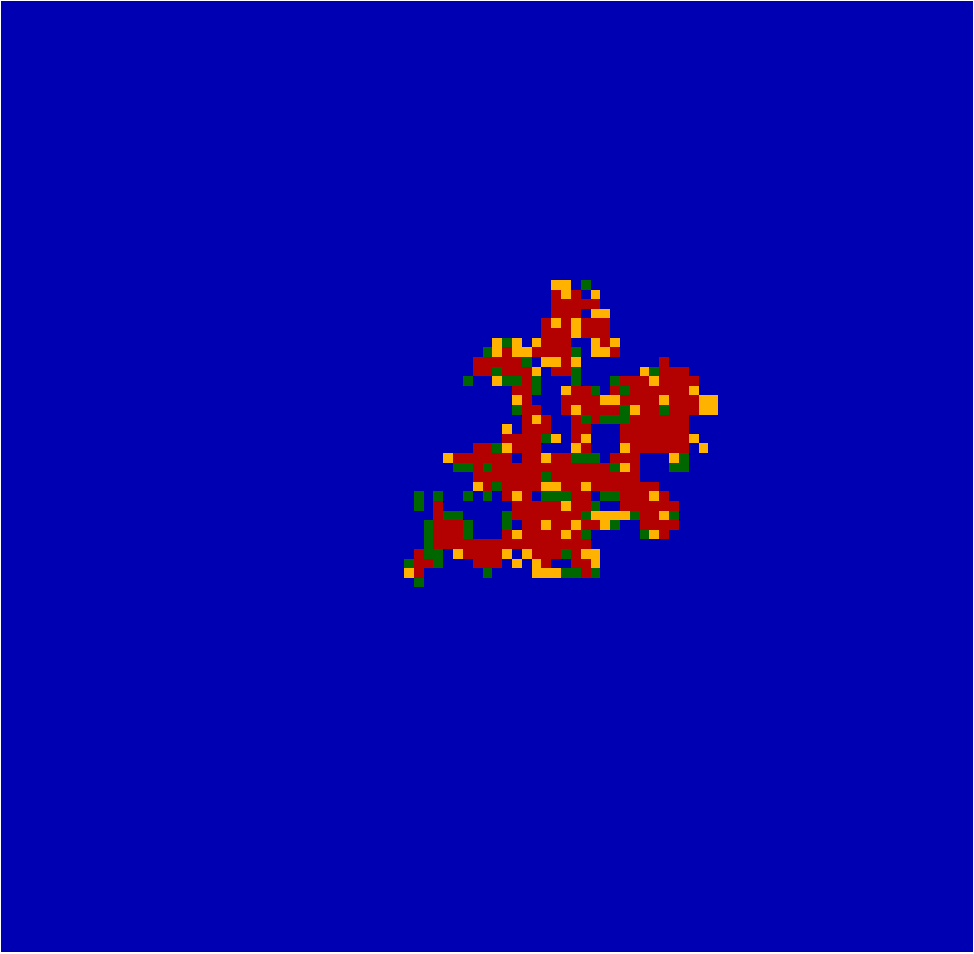
\includegraphics[width=.7\textwidth, angle=0]{./fig/seq_99x99_217steps_MSG_java.png}
			\caption{sequential}
			\label{fig:pd_seq}
		\end{subfigure}
    	&
		\begin{subfigure}[b]{0.4\textwidth}
			\centering
			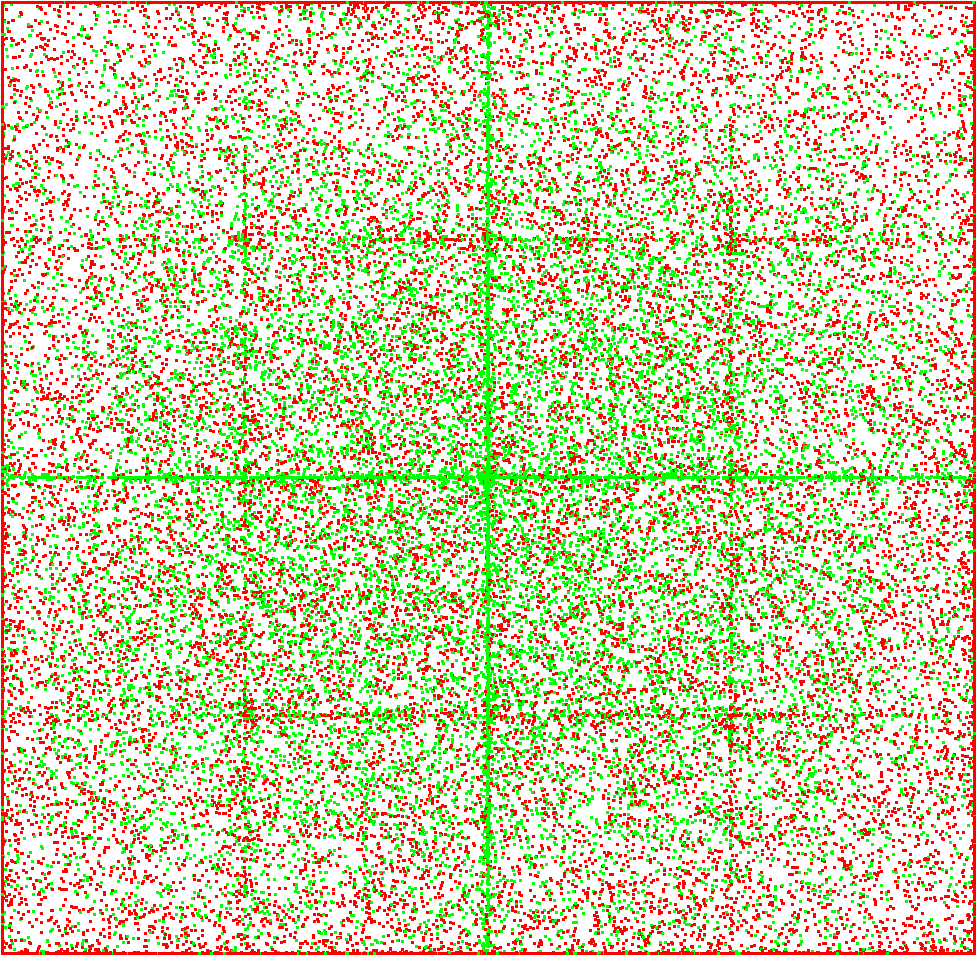
\includegraphics[width=.7\textwidth, angle=0]{./fig/seq_HAC_100_000_500steps_java.png}
			\caption{sequential}
			\label{fig:hac_seq}
		\end{subfigure}
    	\\
    	
    	%\textit{\rotatebox{90}{parallel strategy}}
		
		\begin{subfigure}[b]{0.4\textwidth}
			\centering
			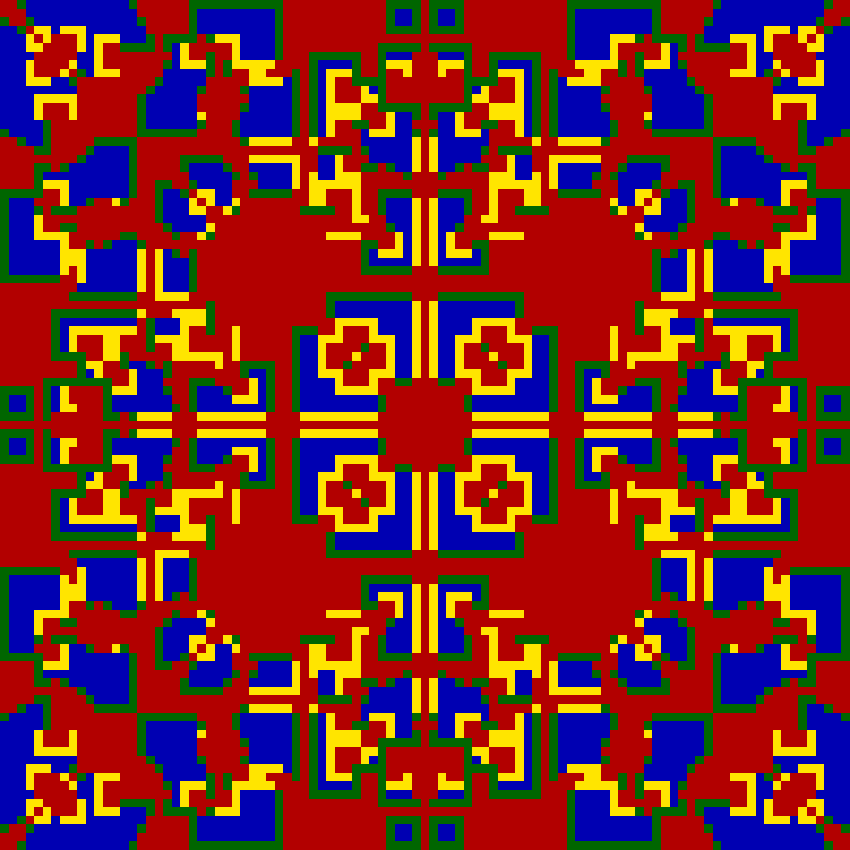
\includegraphics[width=.7\textwidth, angle=0]{./fig/par_99x99_436steps_MSG_haskell.png}
			\caption{parallel}
			\label{fig:pd_par}
		\end{subfigure}
    	&
		\begin{subfigure}[b]{0.4\textwidth}
			\centering
			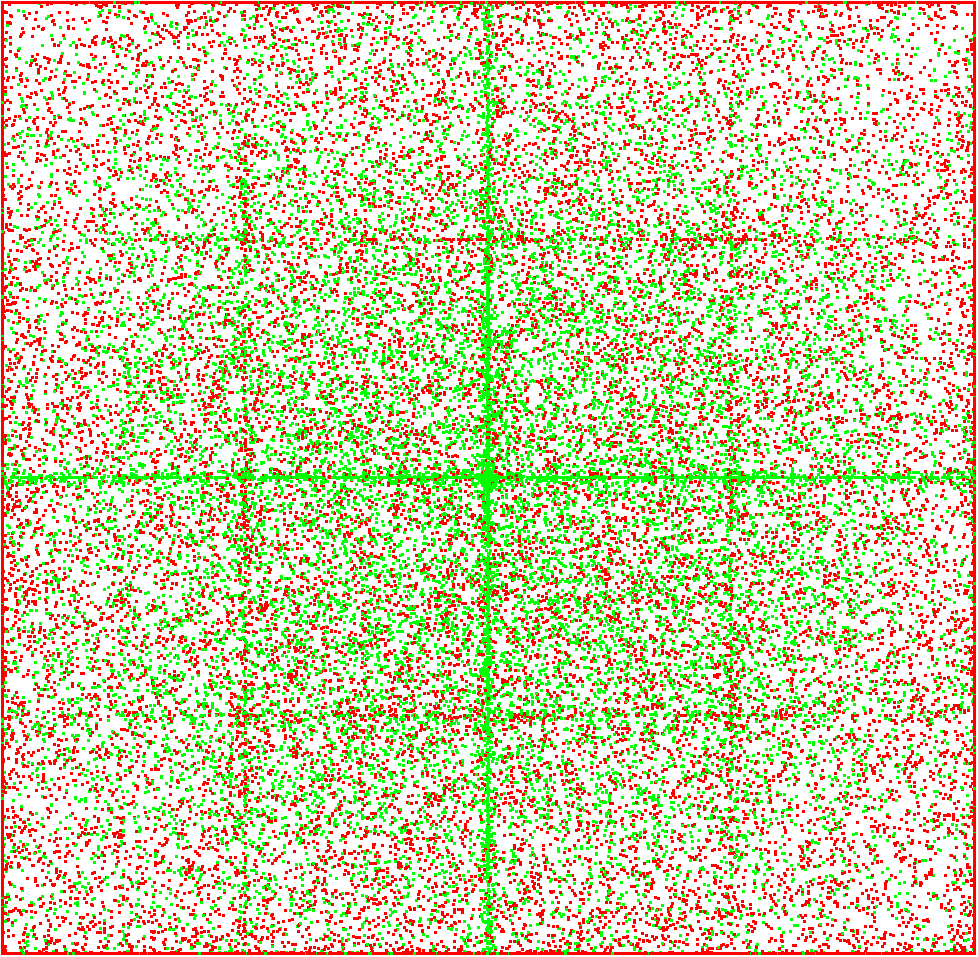
\includegraphics[width=.7\textwidth, angle=0]{./fig/par_HAC_100_000_500steps_java.png}
			\caption{parallel}
			\label{fig:hac_par}
		\end{subfigure}
    	\\
    	
    	%\textit{\rotatebox{90}{concurrent strategy}}
		
		\begin{subfigure}[b]{0.4\textwidth}
			\centering
			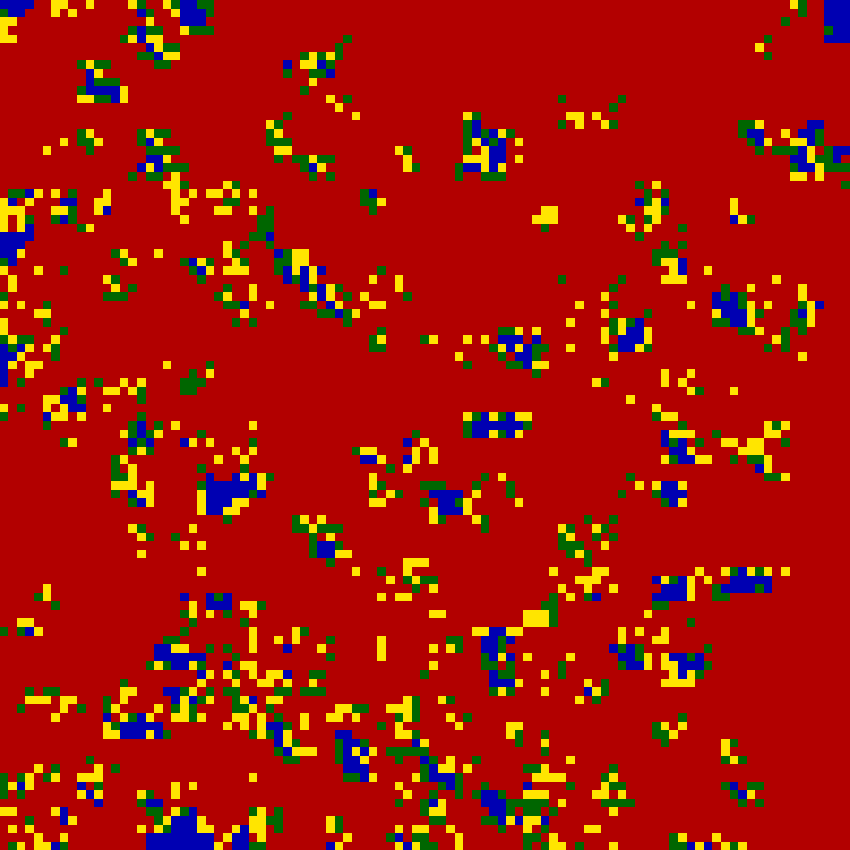
\includegraphics[width=.7\textwidth, angle=0]{./fig/con_99x99_436steps_MSG_haskell.png}
			\caption{concurrent}
			\label{fig:pd_con}
		\end{subfigure}
    	&
		\begin{subfigure}[b]{0.4\textwidth}
			\centering
			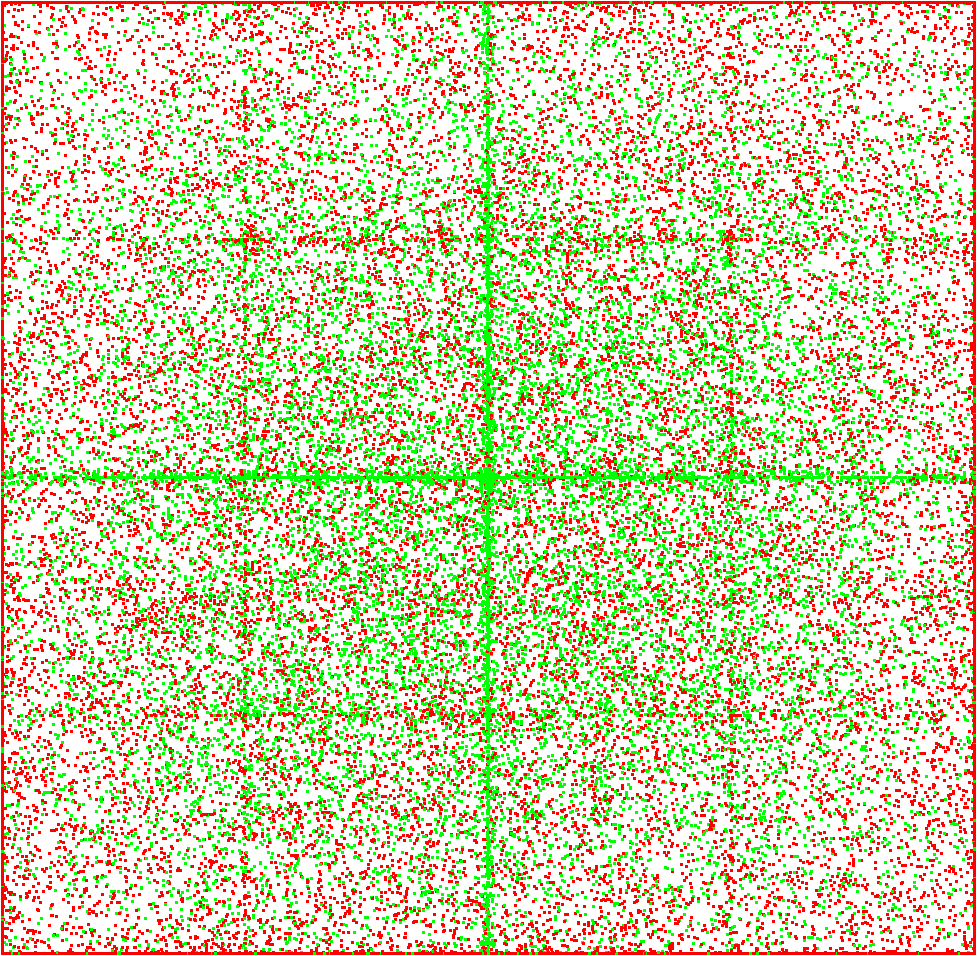
\includegraphics[width=.7\textwidth, angle=0]{./fig/con_HAC_100_000_500steps_java.png}
			\caption{concurrent}
			\label{fig:hac_con}
		\end{subfigure}
    	\\ 
    	
    	%\textit{\rotatebox{90}{actor strategy}}
		
		\begin{subfigure}[b]{0.4\textwidth}
			\centering
			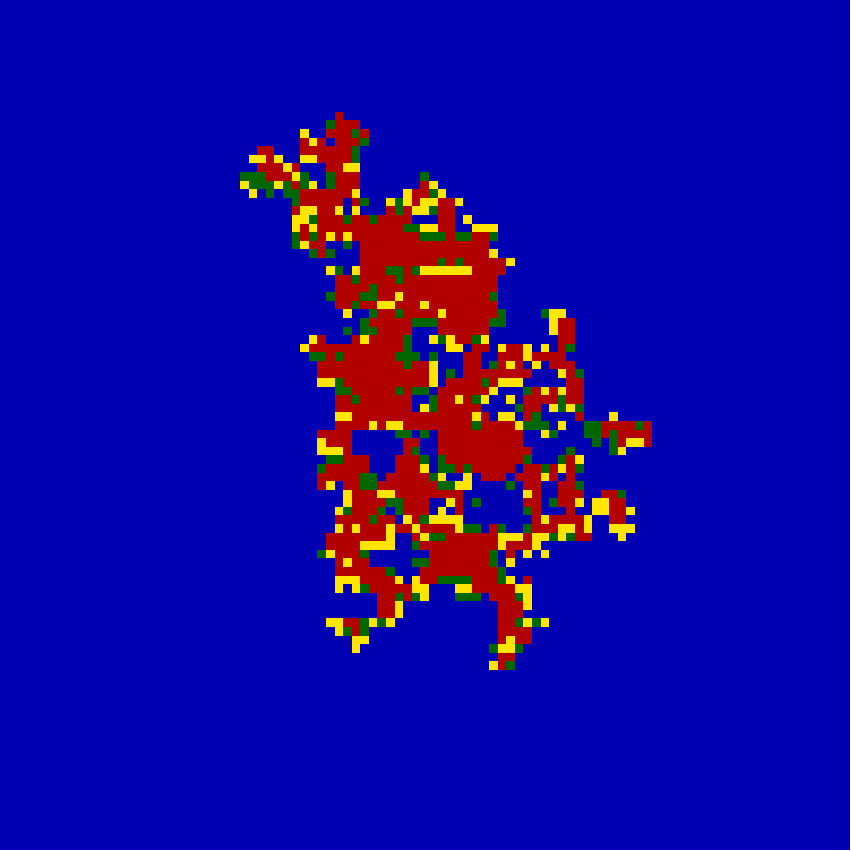
\includegraphics[width=.7\textwidth, angle=0]{./fig/act_99x99_436steps_MSG_haskell.png}
			\caption{actor}
			\label{fig:pd_act}
		\end{subfigure}
    	& 
		\begin{subfigure}[b]{0.4\textwidth}
			\centering
			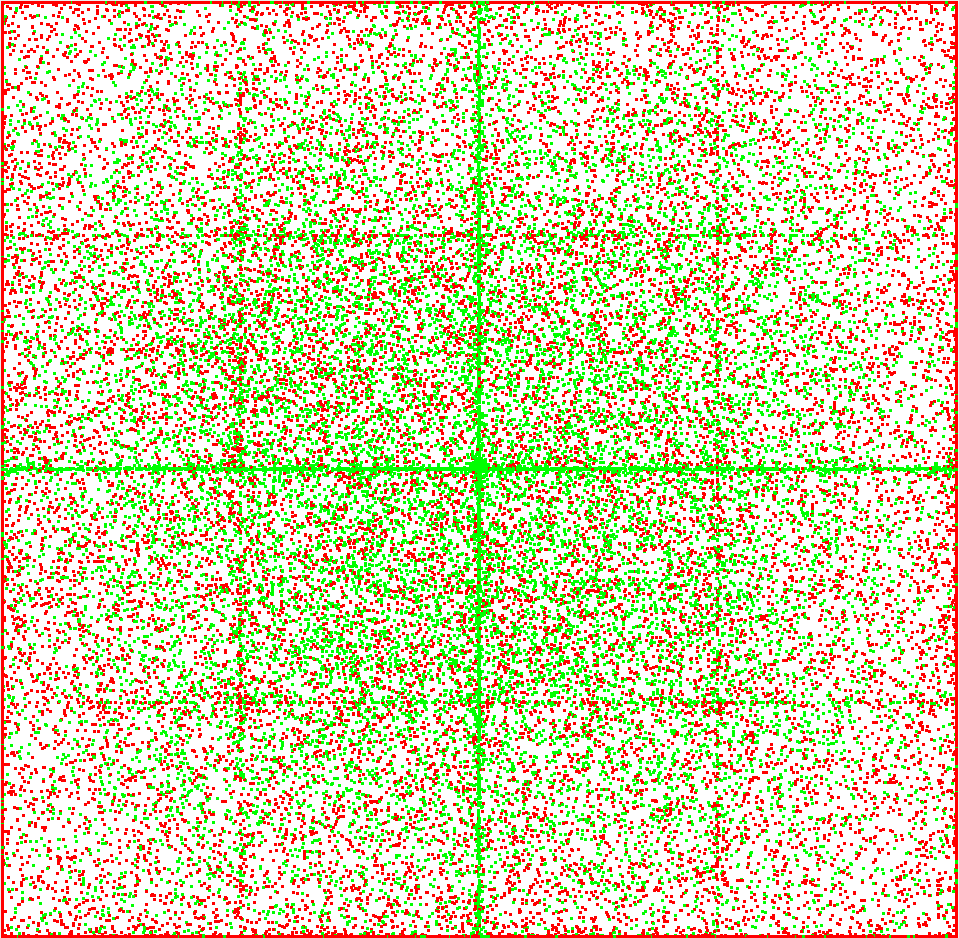
\includegraphics[width=.7\textwidth, angle=0]{./fig/act_HAC_100_000_500steps_scala.png}
			\caption{actor}
			\label{fig:hac_act}
		\end{subfigure}

	\end{tabular}
	
	\caption{\small Effect on results simulating the Prisoners Dilemma and Heroes \& Cowards with all four update-strategies.} 
	\label{fig:results}
\end{table*}

%\begin{figure*}
%
%	 \centering
%	
%    \begin{subfigure}[b]{0.4\textwidth}
%			\centering
%       	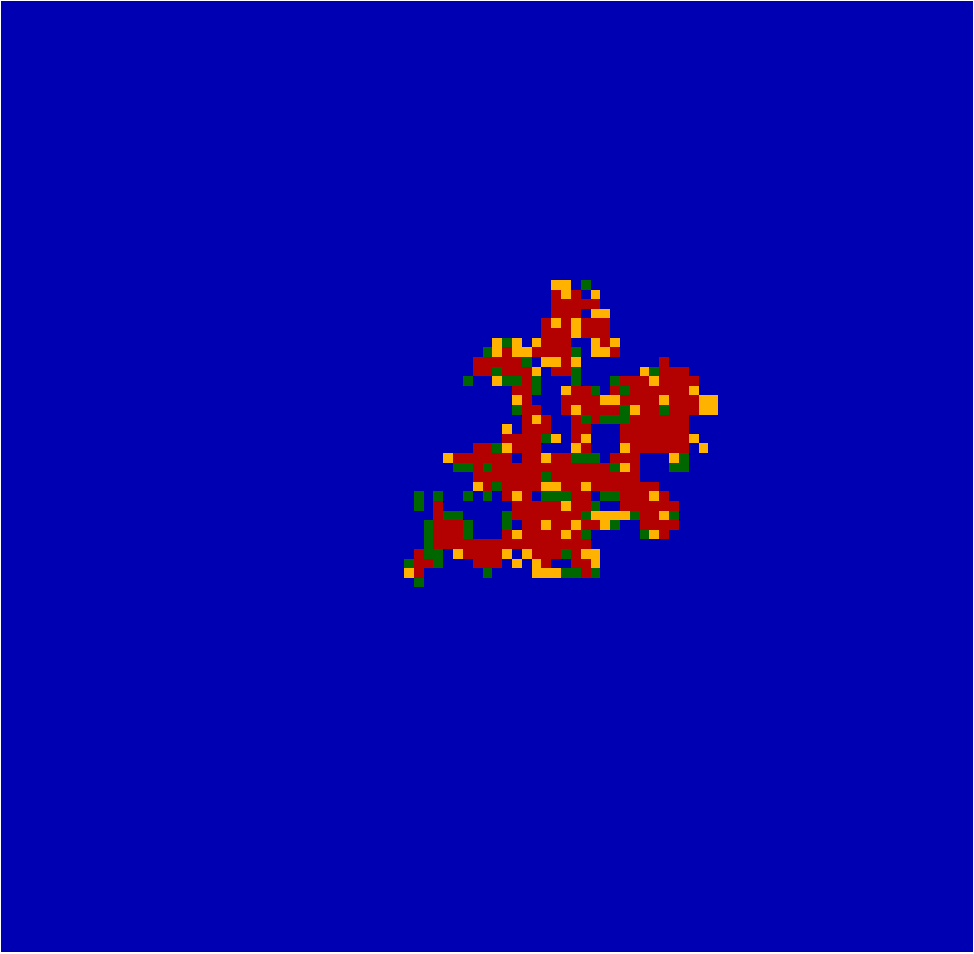
\includegraphics[width=.7\textwidth, angle=0]{./fig/seq_99x99_217steps_MSG_java.png}
%        \caption{\textit{sequential} Prisoners Dilemma}
%        \label{fig:pd_seq}
%    \end{subfigure}
%    \begin{subfigure}[b]{0.4\textwidth}
%		\centering
%        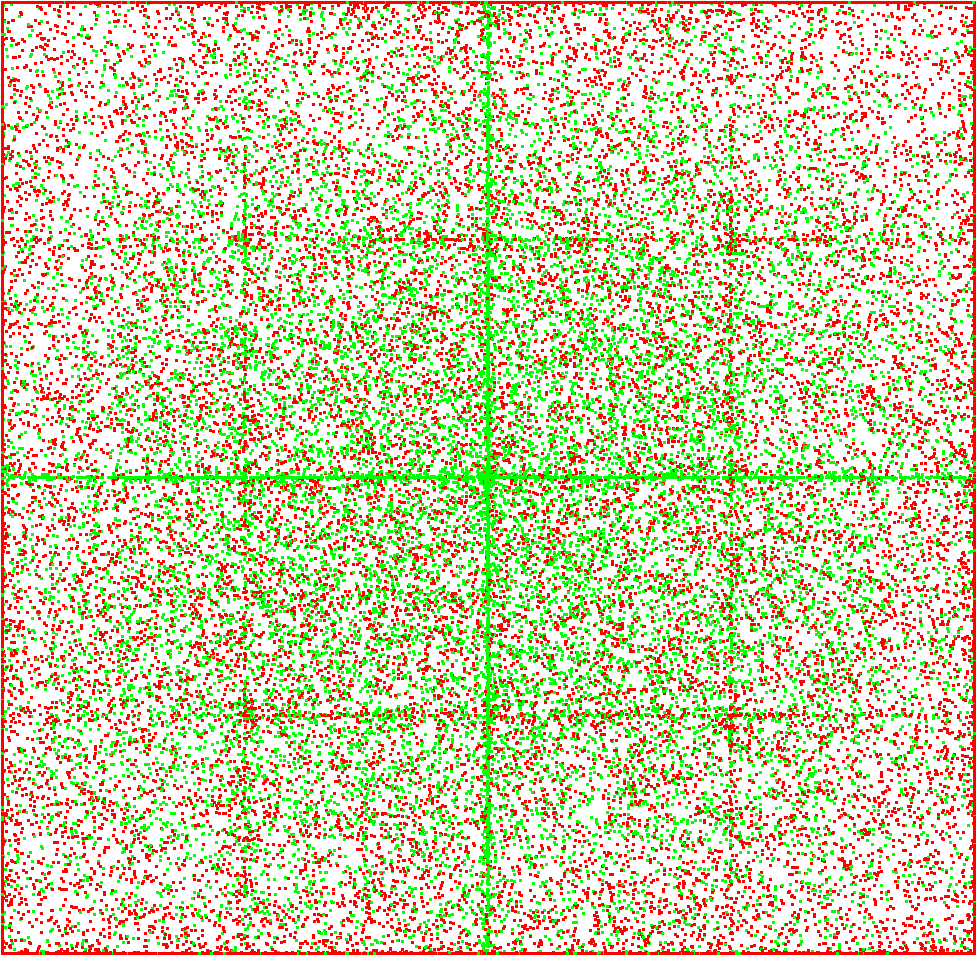
\includegraphics[width=.7\textwidth, angle=0]{./fig/seq_HAC_100_000_500steps_java.png}
%        \caption{\textit{sequential} Heroes \& Cowards}
%        \label{fig:hac_seq}
%    \end{subfigure}
%       
%
%    \begin{subfigure}[b]{0.4\textwidth}
%		\centering
%       	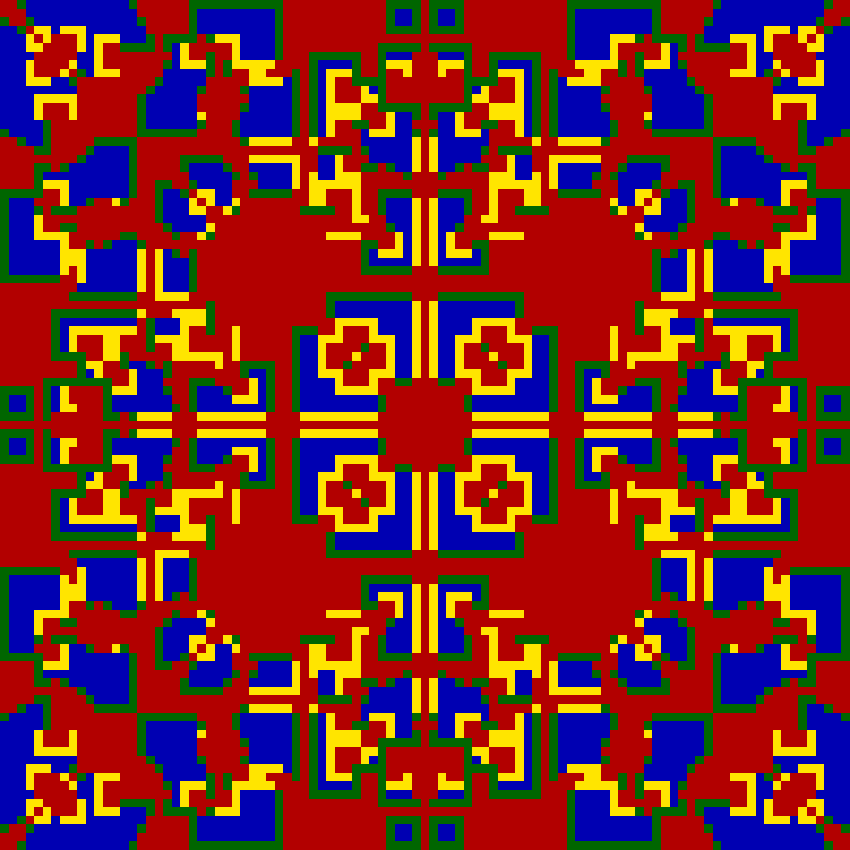
\includegraphics[width=.7\textwidth, angle=0]{./fig/par_99x99_436steps_MSG_haskell.png}
%        \caption{\textit{parallel} Prisoners Dilemma}
%        \label{fig:pd_par}
%    \end{subfigure}
%    \begin{subfigure}[b]{0.4\textwidth}
%    	\centering
%        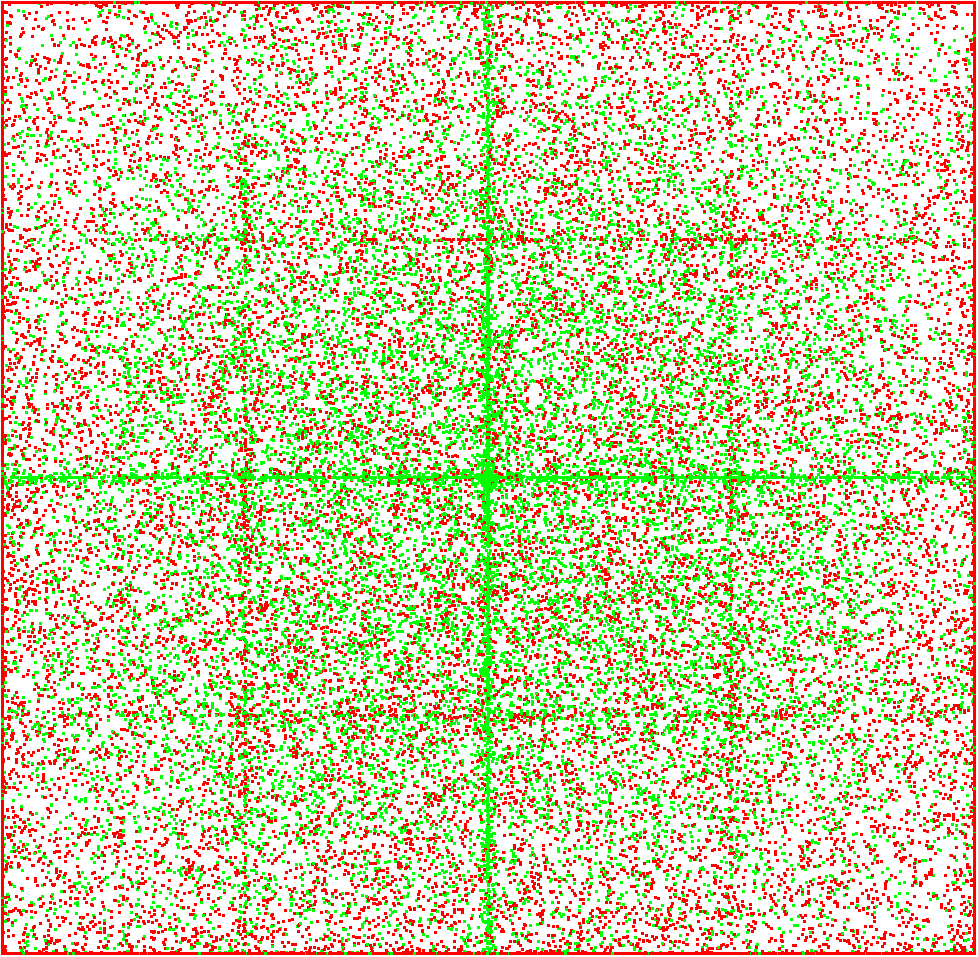
\includegraphics[width=.7\textwidth, angle=0]{./fig/par_HAC_100_000_500steps_java.png}
%        \caption{\textit{parallel} Heroes \& Cowards}
%        \label{fig:hac_par}
%    \end{subfigure}
%        
%
%    \begin{subfigure}[b]{0.4\textwidth}
%		\centering
%       	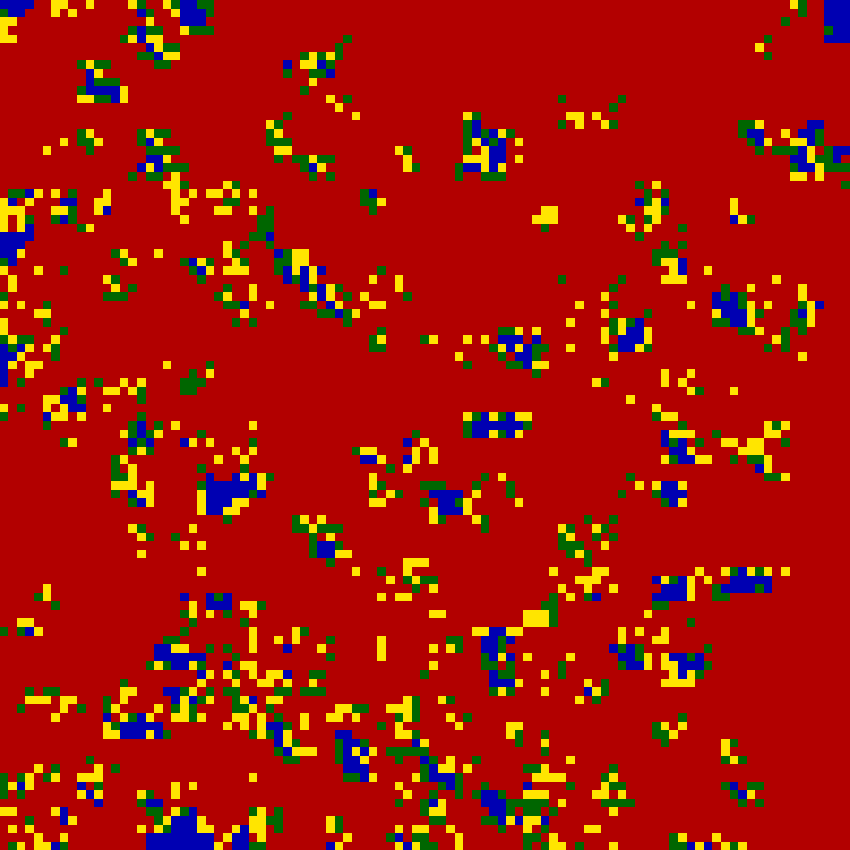
\includegraphics[width=.7\textwidth, angle=0]{./fig/con_99x99_436steps_MSG_haskell.png}
%        \caption{\textit{concurrent} Prisoners Dilemma}
%        \label{fig:pd_con}
%    \end{subfigure}
%    \begin{subfigure}[b]{0.4\textwidth}
%    	\centering
%        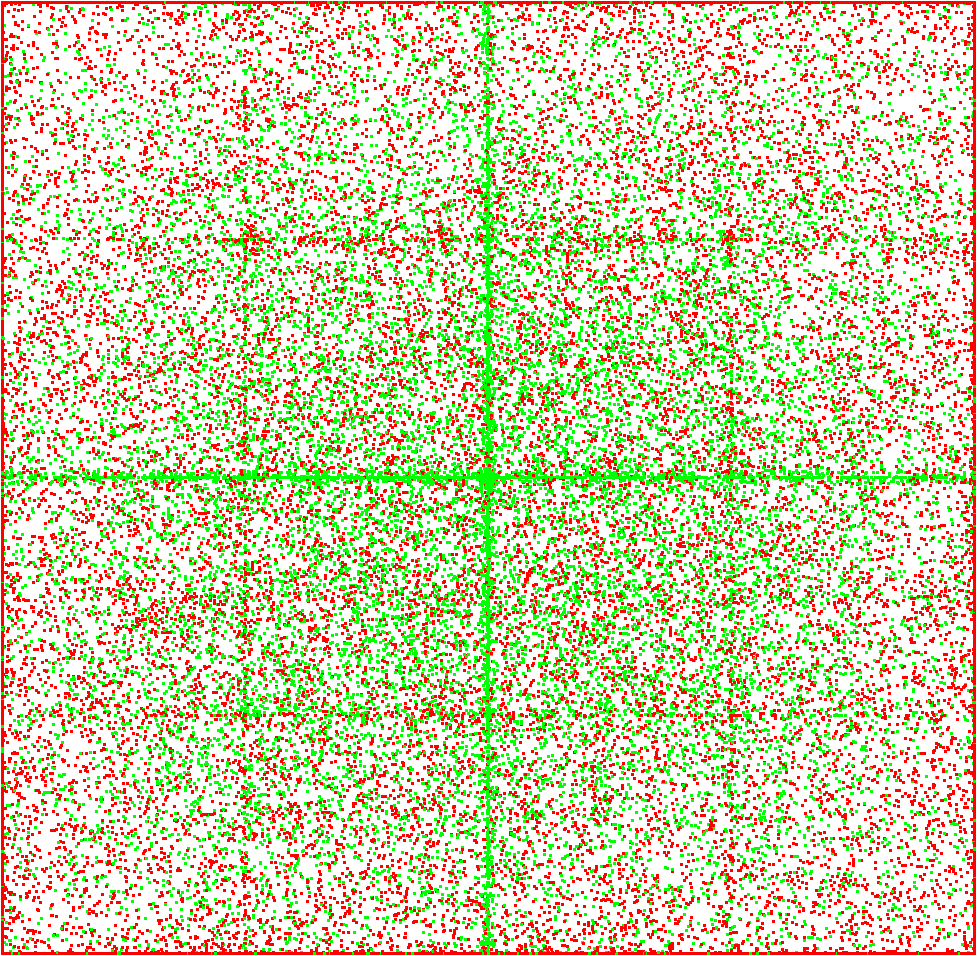
\includegraphics[width=.7\textwidth, angle=0]{./fig/con_HAC_100_000_500steps_java.png}
%        \caption{\textit{concurrent} Heroes \& Cowards}
%        \label{fig:hac_con}
%    \end{subfigure}
%
%
%    \begin{subfigure}[b]{0.4\textwidth}
%		\centering
%       	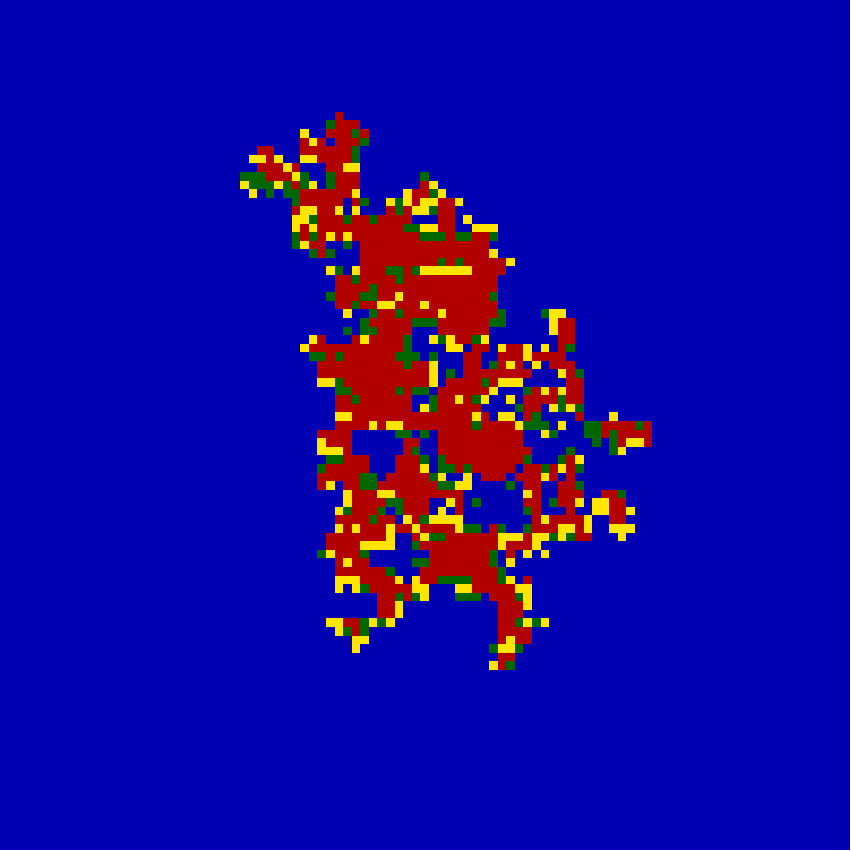
\includegraphics[width=.7\textwidth, angle=0]{./fig/act_99x99_436steps_MSG_haskell.png}
%        \caption{\textit{actor} Prisoners Dilemma}
%        \label{fig:pd_act}
%    \end{subfigure}  
%    \begin{subfigure}[b]{0.4\textwidth}
%    	\centering
%        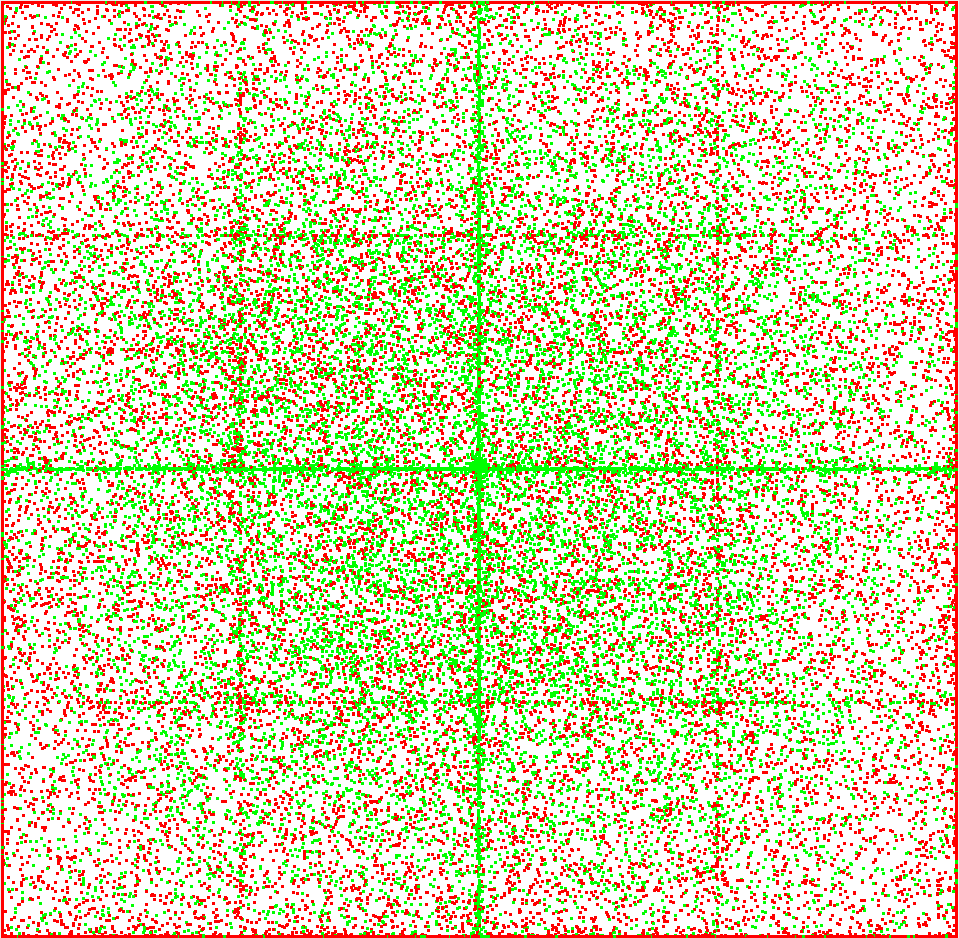
\includegraphics[width=.7\textwidth, angle=0]{./fig/act_HAC_100_000_500steps_scala.png}
%        \caption{\textit{actor} Heroes \& Cowards}
%        \label{fig:hac_act}
%    \end{subfigure}
%
%	\caption{\small Effect on results simulating the Prisoners Dilemma and Heroes \& Cowards with all four update-strategies.} 
%	\label{fig:results}
%\end{figure*}

\subsection{Prisoners Dilemma}
\subsubsection{The agent-based model}
The agent-based model of this game works as follows: an agent sends its state to all its neighbours which allows to incrementally calculate the local payoff. If all neighbours have sent their state then the agent will send its local payoff to all neighbours which allows to compare all payoffs in its neighbourhood and calculate the best. When all neighbours have sent their local payoff the agent will adopt the role of the highest payoff.

\subsubsection{Results}
The results as seen in the left column of figure \ref{fig:results} were created with the same configuration as reported in the original paper: a 99x99 grid with all cooperators except one defector at the center, running for 217 steps. When comparing the pictures with the one from the original paper seen in figure \ref{fig:sync_patterns} the only update-strategy which is able to reproduce the matching result is the \textit{parallel strategy} - all the others clearly fail to reproduce the pattern. From this we can deduce that only the \textit{parallel strategy} is suitable to simulate this model because only that strategy is the one which renders the results of the original paper, meaning it is the 'correct' strategy for this model. The reason why the other strategies fail to reproduce the pattern is due to the non-parallel and unsynchronized way that information spreads through the grid. In the \textit{sequential strategy} the agents further ahead in the queue play the game earlier and influence the neighbourhood so agents which play the game later find already messages from earlier agents in their queue thus acting differently based upon these informations. In the \textit{concurrent} and \textit{actor strategy} the agents run in parallel but changes are visible immediately and concurrently, leading to the same non-structural patterns as in the \textit{sequential} one. This is not the case in the \textit{parallel strategy}  where, in every step, all agents play the game at the same time based on the frozen state of the previous step, leading to a synchronized update as required by the model. Note that the \textit{concurrent} and \textit{actor strategy} produce different results on every run due to the inherent non-deterministic event-ordering introduce by concurrency. As there are no global time-steps in the \textit{actor strategy}, to calculate 217 steps we just waited until the first agent arrived at a local time of 217 and then rendered the result.
Note that when having queued messages instead of immediate messaging in the \textit{sequential strategy} we will end up with the same results as in the \textit{parallel} version. TODO: WHY? TODO: the real difference between SEQ and PAR is that SEQ with immediate messaging changes agents while iterating over the collection, and although the agents don't change unless all their neighbours have answered, this does not guarantee a synchronized update of all agents but only the one because every agent has a different neighbourhood: neighbourhood is reflexive but not transitive: if agent A is in agents B neighbour and agent c is agent bs neighbour this does not imply that agent a is agent c neighbour as well. as agent b receives the final payoff message from agent A and changes its state, 

Also note that in the \textit{parallel strategy} an agent cannot reply to a message within the same step which requires twice as many steps to achieve the same results as in the original paper as seen in figure \ref{fig:sync_patterns}.

\subsection{Heroes \& Cowards}
\subsubsection{The agent-based model}
The agent-based model of this game works as follows: in each time-step an agent asks its friend and enemy for their positions which will answer with a corresponding message containing their current positions. The agent will then have its own local information about the position of its friend and enemy and will calculate its step based on this local information.

\subsubsection{Results}
The results as seen in the right column of figure \ref{fig:results} were created with 100.000 agents where 25\% of them are heroes running for 500 steps. Although the individual agent-positions of runs with the same configuration differ between update-strategies the cross-patterns are forming in all four update-strategies. For the patterns to emerge it is important to have significant more cowards than heroes and to have agents in the tens of thousands - we went for 100.000 because then the patterns are really prominent. We can conclude that the \textit{Heroes \& Cowards} model seems to be robust to the selection of its update-strategy and that its emergent property - the formation of the cross - is stable under differing strategies.